\documentclass[letterpaper,12pt,oneside]{book}  
%\usepackage[a4paper,includeall,bindingoffset=0cm,margin=2cm,marginparsep=0cm,marginparwidth=0cm]{geometry}
\usepackage[top=1in, left=0.9in, right=1.25in, bottom=1in]{geometry}
\usepackage{bachelorstitlepageUNAM}
\usepackage[utf8]{inputenc}
\newcommand{\titulo}{La volatilidad de un activo como movimiento browniano fraccionario}
\newcommand{\autor}{Víctor Miguel García Sánchez}
\usepackage[pdftex]{hyperref}
\hypersetup{
	colorlinks=true,
	linkcolor=black,
	citecolor=black,
	urlcolor=black,
	pdftitle=\titulo, 
	pdfauthor=\autor,
	pdfsubject=Tesis de Maestría,
	pdfkeywords={ponderadores, calibración, información auxiliar, consistencia, inferencia basada en diseño, estimador por regresión, no respuesta, diseño de muestreo complejo}
}
\usepackage{nomencl}
\usepackage{amssymb}
\usepackage{etoolbox}
\usepackage{amsmath}
\usepackage{amsthm}
\usepackage{url}
\usepackage{listings}			%Para incluir código
\lstset{language=R,
	extendedchars=true,
	basicstyle=\ttfamily,
	keywordstyle=\color{blue}\ttfamily,
	commentstyle=\color{gray}\ttfamily,%green
	frame=single, 
	breaklines=true,
	literate=%
		{á}{{\'a}}1
		{é}{{\'e}}1
		{í}{{\'i}}1
		{ó}{{\'o}}1
		{ú}{{\'u}}1
		{ñ}{{\~n}}1
		{Á}{{\'A}}1
		{É}{{\'E}}1
		{Í}{{\'I}}1
		{Ó}{{\'O}}1
		{Ú}{{\'U}}1
		{Ñ}{{\~N}}1
}
\usepackage{appendix}			%Para el índice
\usepackage[font=small,labelfont=bf]{caption}
\usepackage{cleveref}
\crefformat{equation}{ecuación~(#2#1#3)}
\crefformat{theorem}{teorema~(#2#1#3)}
\crefformat{lem}{lema~(#2#1#3)}
\crefformat{item}{inciso~(#2#1#3)}     %Revisar
\crefformat{section}{sección~#2#1#3}
\crefformat{chapter}{capítulo~#2#1#3}
\crefformat{figure}{figura~#2#1#3}
\crefmultiformat{figure}{figuras~#2#1#3}{ y~#2#1#3}{, #2#1#3}{ y~#2#1#3}
\crefmultiformat{equation}{ecuaciones~#2#1#3}{ y~#2#1#3}{, #2#1#3}{ y~#2#1#3}
\crefformat{appendix}{anexo~#2#1#3}
\makenomenclature
\renewcommand{\nomname}{Notación}
\renewcommand{\qedsymbol}{$\blacksquare$}
%%%%%%%%%%%%%%%%%%%%%%%%%%%%%
% Comparto una plantilla para la PORTADA que us\'e en mi t\'esis
% basada en el dise\~no gen\'erico que se usa en la Facultad de Ciencias
% Para usarlo \'unicamente aseg\'urate de tener la l\'inea
% \usepackage{bachelorstitlepageUNAM} y el archivo bachelorstitlepageUNAM.sty en el mismo directorio de trabajo.
% y los campos (sin signo %) :

%Empieza en página par los capítulos
\makeatletter
\renewcommand*{\cleardoublepage}{\clearpage\if@twoside \ifodd\c@page\else
\hbox{}%
\thispagestyle{empty}%
\newpage%
\if@twocolumn\hbox{}\newpage\fi\fi\fi}
\makeatother

\usepackage{epigraph}			%Para la cita al inicio
%Para citas epigráficas
\makeatletter
\renewcommand{\@epirule}{{\rule[.5ex]{\epigraphwidth}{\epigraphrule}}}
\makeatother

%-----------------------__--------

\usepackage[T1]{fontenc}
\usepackage[spanish,es-nodecimaldot,es-tabla]{babel}
\usepackage{graphicx}
\usepackage{tikz} 
\usepackage{tocloft}
\graphicspath{{./figs/}}
\usepackage{setspace}

%\usepackage[round]{natbib}
\theoremstyle{plain}
\newtheorem{theorem}{Teorema}[section]
\newtheorem{dfn}[theorem]{Definición}
\newtheorem{cor}[theorem]{Corolario}
\newtheorem{lem}[theorem]{Lema}
\newtheorem{prop}[theorem]{Proposición}
\newtheorem{rmk}[theorem]{Observación}
\newtheorem{exmp}[theorem]{Ejemplo}
\numberwithin{theorem}{section}
\renewcommand\cftsecpresnum{\S}
\renewcommand\cftsubsecpresnum{\S}   

\renewcommand{\appendixtocname}{List of appendices}
\renewcommand{\appendixname}{List of appendices}
\renewcommand{\appendixname}{Anexos}
\renewcommand{\appendixtocname}{Anexos}
\renewcommand{\appendixpagename}{Anexos}
\begin{document}
%------------------------------
    \begin{titlepage}
        \thispagestyle{empty}
        \begin{minipage}[c][0.17\textheight][c]{0.25\textwidth}
            \begin{center}
                
\includegraphics[width=3.5cm, height=3.5cm]{logo-UNAM.png}
            \end{center}
        \end{minipage}
        \begin{minipage}[c][0.195\textheight][t]{0.75\textwidth}
            \begin{center}
                \vspace{0.3cm}
                \textsc{\large Universidad Nacional Aut\'onoma de M\'exico}\\[0.5cm]
                \vspace{0.3cm}
                \hrule height2.5pt
                \vspace{.2cm}
                \hrule height1pt
                \vspace{.8cm}
                \textsc{Instituto de Investigaciones en Matemáticas Aplicadas y en Sistemas}\\[0.5cm] %
            \end{center}
        \end{minipage}
        \begin{minipage}[c][0.81\textheight][t]{0.25\textwidth}
            \vspace*{5mm}
            \begin{center}
                \hskip2.0mm
                \vrule width1pt height13cm 
                \vspace{5mm}
                \hskip2pt
                \vrule width2.5pt height13cm
                \hskip2mm
                \vrule width1pt height13cm \\
                \vspace{5mm}
                
\includegraphics[height=4.0cm]{logo-IIMAS.png}
            \end{center}
        \end{minipage}
        \begin{minipage}[c][0.81\textheight][t]{0.75\textwidth}
            \begin{center}
                \vspace{1cm}

                {\large\scshape \titulo}\\[.2in]

                \vspace{2cm}            

                \textsc{\LARGE T\hspace{1.5cm}E\hspace{1.5cm}S\hspace{1.5cm}I\hspace{1.5cm}S}\\[0.5cm]
                \textsc{\large que para obtener el t\'itulo de:}\\[0.5cm]
                \textsc{\large Maestro en Ciencias Matemáticas}\\[0.5cm]
                \textsc{\large presenta:}\\[0.5cm]
                \textsc{\large {\autor}}\\[2cm]          

                \vspace{0.5cm}

                {\large\scshape Tutor:\\[0.3cm] {Dr. Arnaud Charles Leo Jegousse}}\\[.2in]

                \vspace{0.5cm}

                \large{Ciudad de México,}{ }{2020}
            \end{center}
        \end{minipage}
    \end{titlepage}
%---------------------------------
            %Notación
\addcontentsline{toc}{chapter}{Notación}
\renewcommand\nomgroup[1]{%
\item[\bfseries
 \ifstrequal{#1}{S}{Símbolos}{%
  \ifstrequal{#1}{T}{Terminología}{%
  \ifstrequal{#1}{Y}{Abreviaturas}{}}}%
]}
%\textsl{volatilidad estocástica fraccionaria}
\nomenclature[Y]{$FSV$}{Modelo de volatilidad estocástica fraccionaria}
\nomenclature[Y]{$RFSV$}{Modelo de volatilidad estocástica fraccionaria áspera}
\nomenclature[Y]{$H$}{Coeficiente de Hurst}
\nomenclature[S]{$\buildrel L^m\over\simeq $}{Igualdad en $L^m$}
\nomenclature[S]{$\buildrel \mathbb P\over\simeq $}{Igualdad en probabilidad}
\nomenclature[S]{$\buildrel d\over\simeq $}{Igualdad en distribución}
\nomenclature[Y]{Bm}{Movimiento Browniano}
\nomenclature[Y]{fBm}{Movimiento Browniano fraccionario}
\nomenclature[S]{$\mathcal V_p$}{La $p-$variación de un proceso}
\nomenclature[Y]{ATM}{At-the-money, en el dinero}
%\nomenclature[T]{$1$}{Inlet}
\nomenclature[T]{log-precio}{Precio en escala logarítmica}
\nomenclature[Y]{$SPX$}{Standard \& Poor's 500 Index, es un índice ponderado por capitalización.}
\nomenclature[Y]{$VIX$}{Chicago Board Options Exchange Market Volatility Index, es un índice que suele coincidir con mínimos en el índice de referencia, regularmente el SPX.}
\nomenclature[Y]{$ATM$}{At-The-Money, es una opción cuyo strike es igual al precio al contado del subyacente}
\nomenclature[T]{spot}{Mercado spot, aquel donde todos los activos que se compran o venden se entregan de forma inmediata al precio del momento y no al precio de la entrega.}

\printnomenclature

\mbox{}
\frontmatter
%\maketitle
\chapter*{}
\begin{flushright}%
  \emph{Dedicado a mi familia, amigos y maestros:\\
gracias a ellos he llegado hasta aquí.}
  \thispagestyle{empty}
\end{flushright}
\chapter{Agradecimientos}
\spacing{1.5}%\doublespacing

\chapter*{Resumen}
\addcontentsline{toc}{chapter}{Resumen}
Un proceso gaussiano $W^H$ es un movimiento Browniano fraccionario (fBm) si es autosimilar de parámetro $H\in(0,1)$, llamado parámetro de Hurst, y tiene incrementos estacionarios. La covarianza en los incrementos de tal proceso está dada por
	\begin{equation}
		\mathbb E(W^H_tW^H_s)=\frac{1}{2}(t^{2H}+s^{2H}+|t-s|^{2H}).
	\end{equation}
Si $H>\frac{1}{2}$, entonces $W^H$ tiene incrementos correlacionados positivamente y decimos que $W^H$ posee memoria larga. Por otro lado, si $H<\frac{1}{2}$, entonces $W^H$ tiene incrementos correlacionados negativamente. Este último caso puede usarse para describir sistemas que cuentan con memoria y persistencia, aunque no tendrá la suavidad que caracteriza al modelo con $H>\frac{1}{2}$ en el que, por el contrario, diremos que es áspero. 

Tras definir la integral estocástica respecto al fBm, es posible desarrollar la teoría necesaria para enunciar una versión fraccionaria de la fórmula de Itô. Además, al denotar la relación de tal integral estocástica con la integral estocástica respecto al movimiento Browniano (Bm) estandar, es posible bajo ciertas condiciones hablar de una versión fraccionaria del Teorema de Girsanov. La fórmula de Itô y el Teorema de Girsanov son muy importantes en la teoría de finanzas matemáticas, así que la existencia de versiones fraccionarias para los mismos, es un buen indicio de la incorporación del modelo de fBm para usos prácticos.

En \cite{gatheral_volatility_2018} se define al modelo de volatilidad estocástica fraccionaria áspera (RFSV) usando un fBm con $H <\frac{1}{2}$, que tiene el potencial para satisfacer las propiedades observadas empíricamente en las series de tiempo de la volatilidad de precios de activos.

Cuando se estima la volatilidad con datos de alta frecuencia, se verifica la suavidad del proceso de volatilidad. Además observamos que el modelo RFSV es consistente con los datos financieros de series de tiempo; una aplicación es que nos permite obtener pronósticos mejorados de la volatilidad. Además encontramos que aunque la volatilidad no es un proceso de memoria larga en el modelo RFSV, los procedimientos estadísticos clásicos que apuntan a detectar la persistencia de la volatilidad, tienden a concluir la presencia de memoria larga en los datos generados a partir de ella, reafirmando la utilidad del modelo en la práctica.

\textcolor{red}{Está escrito a la fecha, falta extender}
\newpage
\tableofcontents
%6.1Integrals with respect to fBm. . . . . . . . . . . . . . . . . . . . . . . . . . . . . . . . . . . . . . . . . 147
%biagini
\newpage
\listoffigures
\listoftables
\mainmatter
\chapter*{Introducción}
\addcontentsline{toc}{chapter}{Introducción}
\epigraph{\textsl{La volatilidad implícita es el ‘número incorrecto utilizado en la fórmula incorrecta para obtener el precio correcto'.}}{\textit{\textbf{Riccardo  Rebonato}\\ Theory and Practice of Model Risk Management.(1999)}}
\section*{Justificación}
\addcontentsline{toc}{section}{Justificación}
En la actualidad se necesitan profesionales en el sector financiero, en el cual se prefieren la modelación sobre la simulación, ya que la modelación justifica de mejor manera las aplicaciones prácticas del análisis técnico financiero.

El modelo más utilizado para estudiar el comportamiento financiero es el de Black-Scholes, propuesto en \cite{black_pricing_1973-1}, a partir del cual se ha desarrollado una buena parte de la teoría de las finanzas matemáticas, sin embargo una de las principales características de este modelo, expuesto en la \ref{ec1.2} es que su volatilidad $\sigma$ es constante, comportamiento que solo se presenta localmente en la realidad.

Estudiaremos en contraste un modelo de volatilidad estocástica, justificado por la evidencia hallada en datos del \textsl{VIX} (Chicago Board Options Exchange Market Volatility Index).
\section*{Antecedentes}
\addcontentsline{toc}{section}{Antecedentes}
En \cite{mandelbrot_fractional_1968},

En \cite{comte_long_1998}, introducen el modelo de \textsl{volatilidad estocástica fraccionaria} (FSV).

En \cite{gatheral_volatility_2018}, consideran el modelo FSV con un exponente de Hurst $H<\frac{1}{2}$, al que cual nombran como modelo de \textsl{volatilidad estocástica fraccionaria áspera} (RFSV). Éste es consistente con datos de series de tiempo financieras.
\section*{Hipótesis}
\addcontentsline{toc}{section}{Hipótesis}
El modelo de volatilidad estocástica fraccionara áspera, inspirado en el fBm con parámetro de Hurst $H<\frac{1}{2}$, representa de mejor manera el comportamiento observado en datos de frecuencia ultra alta, además de poseer la propiedad de memoria larga, que también se ha investigado ampliamente en los estudios de análisis técnico financiero, como en los fenómenos de repetición de patrones, por mencionar un ejemplo.
\section*{Objetivos}
\addcontentsline{toc}{section}{Objetivos}
\subsection*{Objetivos generales}
\addcontentsline{toc}{subsection}{Objetivos generales}
\subsection*{Objetivos específicos}
\addcontentsline{toc}{subsection}{Objetivos específicos}
\section*{Delimitación del problema}
\addcontentsline{toc}{section}{Delimitación del problema}
\section*{Estructura del documento}
\addcontentsline{toc}{section}{Estructura del documento}
\chapter{Preámbulo}%\textcolor{red}{Nombre del capítulo}%????? Ingredientes?
%??En palabras de \cite{mandelbrot_fractional_1968}
\section{La volatilidad}
Para describir el comportamiento del precio de un activo $S_t$, el modelo más usado es el de \cite{black_pricing_1973-1},
\begin{align}\label{ec1.2}
	\frac{dS_t}{S_t}=\mu(t,S_t)dt+\sigma(t)dW_t,
\end{align}
donde $\mu$ es un término de deriva o tendencia y $W_t$ es un Bm estándar. El término $\sigma$ es el proceso de \textbf{volatilidad}, el cual también nos interesa estudiar a escala logarítmica, también llamada \textbf{log-volatilidad}.

En tal modelo, $\sigma$ es constante o una función determinista del tiempo, mientras que en los modelos de volatilidad estocástica, se complexifica el comportamiento de $\sigma$ al darle un comportamiento aleatorio. Uno de los primeros modelos de volatilidad estocástica se tiene en \cite{hull_one-factor_1993}, en el cual $\sigma$ está modelada como una semimartingala browniana continua, cuya dinámica es más realista, pues en este modelo la volatilidad del subyacente, además de variar respecto al tiempo, posee un riesgo específico.

Al modelo \ref{eq1.3} expuesto a continuación lo llamaremos \textbf{modelo de volatilidad estocástica}, donde la log-volatilidad $\ln\sigma(t)$ es un proceso de Ornstein-Uhlenbeck:
\begin{align}\label{eq1.3}
	\left\{\begin{matrix}\frac{dS_t}{S_t}=\mu(t,S_t)dt+\sigma(t)dW_{1,t}\\d(\ln \sigma(t))=k(\theta-\ln \sigma(t))dt+\gamma dW_{2,t} \end{matrix}\right.,
\end{align}
donde $W_1,W_2$ son Bm no degenerados, lo cual asegura que el proceso de volatilidad instantánea sea estacionario, con la finalidad de generalizar la volatilidad constante o determinista del modelo de Black-Scholes a una volatilidad estocástica que, de acuerdo a \cite{hull_one-factor_1993}, posee la volatilidad estocástica observada en la práctica y extiende al modelo de Vasicek propuesto en \cite{hull_pricing_1990}.

En contraste con el modelo expresado en la \cref{ec1.2}, se pueden producir sesgos en la fijación de precios o cobertura de opciones. Tal efecto es conocido en la literatura empírica como el efecto ``\textsl{smile}''. Se cree que los smiles en la volatilidad pueden explicarse mediante los modelos de volatilidad estocástica, que podrían tener en cuenta, entre otras propiedades, el clustering de volatilidad mencionado al final de la \cref{sec1.1.1}.

En términos de la suavidad del proceso de volatilidad, existen dos posibilidades: contar con rutas muy regulares, que es el caso de Black-Scholes, o bien, contar con trayectorias de volatilidad con una regularidad cercana a la del movimiento Browniano, que es el caso de los modelos de volatilidad local y estocástica.
\section{El movimiento Browniano fraccionario}
Nos interesa poder replicar el análisis a distintas escalas de tiempo de interés práctico, que van desde un día hasta varios años. Esta propiedad es llamada \textbf{autosimilitud}, tal nombre se debe a \cite{mandelbrot_fractional_1968}.

%Sean $t\in \mathbb R$ el tiempo, $W_t$ un movimiento Browniano estándar y un parámetro $H\in (0,1)$, llamado parámetro de Hurst. %%eqivalencia:. 7.2.3 stable??
\begin{dfn}\label{Def1.2.1}
Llamemos \textbf{autosimilar de parámetro $H$ ($H\geq0$)} a un proceso estocástico $X=(X_t)$, si para cualesquiera $h>0$ y $t_0$, se cumple que
\begin{align*}
\left(X_{t_0}\right)\buildrel d\over\simeq \left(h^{-H}X_{ht_0}\right)
\end{align*}
\end{dfn}
Proponemos ahora la definición de movimiento Browniano fraccionario (fBm) estándar expuesta en \cite{samorodnitsky_stable_1994}.
\begin{dfn}
Un proceso gaussiano $W^H$ es un \textbf{movimiento Browniano fraccionario} (\textbf{fBm}) si es autosimilar de parámetro $H\in(0,1)$, al que llamaremos parámetro de Hurst, y tiene incrementos estacionarios.
\end{dfn}
Probemos ahora la existencia del fBm, comenzando con las siguientes propiedades:
\begin{lem}\label{lem1.1.3}
	Sea $(X_t)$ un proceso gaussiano autosimilar de parámetro $H$. Entonces,
	\begin{enumerate}
		\item\label{lem1.2.3.1} $X_0\buildrel c.s. \over =0$
		\item\label{lem1.2.3.2} Si $(X_t)$ tiene incrementos estacionarios, entonces al fijar un tiempo $t$, tenemos que $X_{-t}\buildrel d \over\simeq -X_t$
		\item\label{lem1.2.3.3} Para todo $t\in\mathbb R$, se cumple que $\mathbb E[X_t]=0$
		\item\label{lem1.2.3.4} Si además $(X_t)$ es un proceso de varianza finita, entonces para cualesquiera $t_1,t_2\in\mathbb R$,
		$$Cov(X_{t_1},X_{t_2})=\frac{1}{2}\left(|t_1|^{2H}+|t_2|^{2H}-|t_1-t_2|^{2H}\right)Var (X_1)$$
	\end{enumerate}
\end{lem}
\begin{proof}
	\begin{enumerate}
		\item Sea $h>0$ arbitrario. Entonces $X_0\buildrel d \over\simeq h^{H}X_0$, así que $X_0(h^{H}-1)\buildrel d \over\simeq0$.
		
		Como $h$ es arbitrario, entonces $X_0$ casi seguramente es $0$ .
		\item Usando \ref{lem1.2.3.1}, podemos observar que $X_{-t}\buildrel d \over\simeq X_{-t}-X_0$.
		Ya que $(X_t)$ tiene incrementos estacionarios, entonces $X_{-t}\buildrel d \over\simeq X_0-X_t\buildrel d \over\simeq -X_t$.
		\item Veamos que
			\begin{align*}
				\mathbb E[X_1]&=\mathbb E[X_2-X_1]\\
							&=\mathbb E[2^{H}X_1]-\mathbb E[X_1]\\
							&=(2^{H}-1)\mathbb E[X_1],
			\end{align*}
			lo cual implica que $\mathbb E[X_1]=0$.
			
			Sea $t>0$, entonces por la autosimilitud de $(X_t)$, tenemos que $\mathbb E[X_t]=t^{H}\mathbb E[X_1]=0$. Usando \ref{lem1.2.3.2}, podemos extenderlo de forma que la expresión es válida para cada $t\in \mathbb R$.
		\item Por \ref{lem1.2.3.3}, tenemos que
			\begin{align*}
				Cov(X_{t_1},X_{t_2})&=\mathbb E\left[X_{t_1}X_{t_2}\right]\\
								&=\frac{1}{2}\mathbb E\left[X^2_{t_1}+X^2_{t_2}-(X_{t_1}-X_{t_2})^2\right]\\
								&=\frac{1}{2}\left[\mathbb E\left[X^2_{t_1}\right]+\mathbb E\left[X^2_{t_2}\right]-\mathbb E\left[(X_{t_1-t_2}-X_{0})^2\right]\right]\\
								&=\frac{1}{2}\left[\mathbb E\left[X^2_{|t_1|}\right]+\mathbb E\left[X^2_{|t_2|}\right]-\mathbb E\left[X_{|t_1-t_2|}^2\right]\right]\\
								&=\frac{1}{2}\left[|t_1|^{2H}\mathbb E\left[X^2_{1}\right]+|t_2|^{2H}\mathbb E\left[X^2_{1}\right]-|t_1-t_2|^{2H}\mathbb E\left[X_{1}\right]^2\right]\\
								&=\frac{1}{2}(|t_1|^{2H}+|t_2|^{2H}-|t_1-t_2|^{2H})\mathrm{Var}(X_1).
			\end{align*}
	\end{enumerate}
\end{proof}
Un fBm es llamado movimiento Browniano fraccionario \textbf{estándar} si $\mathrm{Var}(X_1)=1$.

Al hecho de que $Var[W^\frac{1}{2}_{t+\tau}-W_t^\frac{1}{2}]=T$ se le conoce también como \textit{Ley $T^{\frac{1}{2}}$}, lo cual es considerado como parte de la definición del movimiento Browniano estándar. Ésta propiedad es generalizada en \cite{coutin_introduction_2007}
de la siguiente manera:
\begin{cor}
	Una ley $T^H$ para la desviación estándar de $W^H$ puede enunciarse como:
	$$\mathbb E[|W^H_{t+T}-W^H_t|^q]=T^{Hq}V_q$$
	donde $V_q=\mathbb E(|N(0,1)|^q)$.
\end{cor}
\begin{proof}
	Usando que el fBm tiene incrementos estacionarios, se sigue que,
	\begin{align*}
		\mathbb E[|W^H_{t+T}-W^H_t|^q]&=\mathbb E[|W^H_{T}|^q],
		\intertext{como $W^H$ es autosimilar de parámetro $H$,}
									&=\mathbb E[|T^{H}W^H_{1}|^q]\\
									&=T^{Hq}\mathbb E[|W^H_{1}|^q]
		\intertext{Además, como $W^H$ es un proceso gaussiano, $\mathbb E[|W^H_{t+T}-W^H_t|^q]=T^{Hq}V_q$}
	\end{align*}
%\textcolor{red}{No se si quitarle más renglones}
\end{proof}
%decir... algo, no solo aventar teoremas
%en el capitulo 1 del diffusions
Cuando $H=\frac{1}{2}$, $W^H$ es el Bm estándar, lo cual se puede ver de su covarianza exhibida en \ref{lem1.2.3.4}, así que es una martingala. Por otro lado, para $H\neq\frac{1}{2}$ no lo es. Para probarlo requerimos introducir la siguiente definición.
\begin{dfn}
	Sean $X$ un proceso estocástico, $\pi_T=\{0=t_0<t_1<\ldots<t_n=T\}$ una partición finita de $[0,T]$ y
	$$\delta(X,\pi_T):=\sum_{i=1}^n\left|X_{t_i}-X_{t_{i-1}}\right|^p.$$
	La $p-$variación de $X$ sobre el intervalo $[0,T]$ está definido como
	$$\mathcal V_p\left(X,[0,T]\right):=\sup_{\pi_T} \delta_p(X,\pi_T)$$
\end{dfn}
\begin{theorem}
	El fBm $W^H$ es una semimartingala si y sólo si $H=\frac{1}{2}$.
\end{theorem}
\begin{proof}$(\Leftarrow)$ Como $W^{\frac{1}{2}}$ es un Bm, entonces es una semimartingala.
	
	$(\Rightarrow)$ Para $p>0$, consideremos las particiones de la forma $\pi_1=\{t_k=\frac{k}{n}:0\leq k\leq n\}$ y definamos
	\begin{align*}
		Y_{n,p}&:=n^{pH-1}\sum_{i=1}^n\left|W^H_{\frac{i}{n}}-W^H_{\frac{i-1}{n}}\right|^p
		\intertext{Como $W^H$ es autosimilar,}
			&\buildrel d \over\simeq n^{pH-1}\sum_{i=1}^nn^{-pH}\left|W^H_{i}-W^H_{i-1}\right|^p\\
			&= n^{-1}\sum_{i=1}^n\left|W^H_{i}-W^H_{i-1}\right|^p\\
			&=:\tilde Y_{n,p}.
	\end{align*}
	Veamos que por el Teorema ergódico,
	$$\lim_{n\rightarrow\infty}\tilde Y_{n,p}=\lim_{n\rightarrow\infty}\frac{\sum_{i=1}^n\left|W^H_{i}-W^H_{i-1}\right|^p}{n}\buildrel L^1 \over\simeq \mathbb E\left[|W^H_1|^p\right]$$
	Luego, como $Y_{n,p}\buildrel d \over\simeq \tilde Y_{n,p}$, entonces
	\begin{align*}
		\lim_{n\rightarrow\infty} n^{pH-1}\sum_{i=1}^n\left|W^H_{\frac{i}{n}}-W^H_{\frac{i-1}{n}}\right|^p&=\lim_{n\rightarrow\infty} \tilde Y_{n,p}\buildrel \mathbb P \over\simeq \mathbb E\left[|W^H_1|^p\right].
\intertext{De aquí que}
\lim_{n\rightarrow\infty}\sum_{i=1}^n\left|W^H_{\frac{i}{n}}-W^H_{\frac{i-1}{n}}\right|^p&\buildrel \mathbb P \over\simeq \lim_{n\rightarrow\infty}n^{1-pH}\mathbb E\left[|W^H_1|^p\right]\\
	&\buildrel \mathbb P \over\simeq
	\left\{\begin{matrix}
			0&\text{ si }pH>1\\
			\mathbb E\left[|W^H_1|^p\right] &\text{ si }pH=1\\
			\infty&\text{ si }pH<1
			\end{matrix}
	\right..
	\end{align*}
	Como consecuencia de lo anterior, tenemos que
	\begin{equation}\label{eq1.1}
		\mathcal V_p\left(W^H,[0,1]\right) \buildrel\mathbb P \over\simeq
		\left\{\begin{matrix}
					0&\text{ si }pH>1\\
					\mathbb E\left[|W^H_1|^p\right] &\text{ si }pH=1\\
					\infty&\text{ si }pH<1
			\end{matrix}
		\right..
	\end{equation}
%	Procedamos ahora por contrapositiva: Supongamos que $W^H$ es una semimartingala.
	\begin{itemize}
		\item Si $H>\frac{1}{2}$, veamos que para $p=2$, tenemos que $pH>1$, así que por la \cref{eq1.1}, se sigue que $\mathcal V_2\left(W^H,[0,1]\right)\buildrel\mathbb P \over\simeq0$. Como $W^H$ tiene incrementos estacionarios, entonces $W^H$ tiene variación cuadrática $0$ en cualquier en intervalo. Procedamos por contradicción:

		Supongamos que $W^H$ es una semimartingala y sea $W^H=M+A$ su descomposición, donde $M=W^H-A$ es una martingala de variación cuadrática $0$, así que es una constante. Como $M$ es constante, entonces $W^H=M+A$ es de variación acotada, es decir $\mathcal V_1\left(W^H,[0,1]\right)<\infty$.
		
		Por otro lado, para $p=1$, la \cref{eq1.1} obtenemos que que $\mathcal V_1\left(W^H,[0,1]\right)\buildrel\mathbb P \over\simeq\infty$. %$\textcolor{red}{No se como concluir este caso, ¿basta con decir que las semimartingalas deben tener variación cuadrática finita distinta de 0? En Biagini 2008 Prop 2.4.5. dice que la 1-variación es infinita}
		La contradicción anterior nos indica que no es posible que $W^H$ sea una semimartingala.
		
		\item Si $H<\frac{1}{2}$, tomemos $p=2$. Como $pH<1$, entonces $\mathcal V_2\left(W^H,[0,1]\right)\buildrel\mathbb P \over\simeq\infty$. %y análogamente al caso anterior, la $p-$variación de $W^H$ es infinita sobre todo intervalo fijo.
		Ya que las semimartingalas tienen variación cuadrática finita, entonces $W^H$ no puede ser una semimartingala.
	\end{itemize}
	Por lo anterior, solo se puede tener $H=\frac{1}{2}$.
\end{proof}
Como la integral estocástica de Itô se define sobre semimartingalas, entonces no es posible definir la integral estocástica respecto a $W^H$ de esta manera,  sin embargo, en \cite{comte_long_1996}, mencionan que solo se requiere la integración en $L^2$ sobre procesos gaussianos para la valuación de opciones.
\subsection{Memoria larga}\label{sec1.1.1}
Para introducir el concepto de memoria larga, el cual se ha refinado a lo largo del tiempo, 
comencemos describiendo la covarianza entre incrementos de tiempo.
\begin{theorem}\label{teo1.2.8}
	Sean $t<s\in \mathbb R$ y $h>0$ el tamaño de los incrementos de tiempo, de forma que $t+h\leq s$. Sea $n=\frac{s-t}{h}\geq1$. Denotemos la covarianza entre incrementos con la notación de \cite{biagini_stochastic_2008}, $\rho_H(n)=Cov\left[W^H_{s+h}-W^H_{s},W^H_{t+h}-W^H_{t}\right]$%\sum_{k=0}^{+\infty}Cov[W^H_1,W^H_k-W^H_{k-1}]$$
, entonces
	\begin{align*}
		\rho_H(n)&=h^{2H}\left[\frac{(n+1)^{2H}+(n-1)^{2H}}{2}-n^{2H}\right] Var(W^H_1)
	\end{align*}
\end{theorem}
\begin{proof}
	Veamos que
	\begin{align*}
		\rho_H(n)&=Cov\left[W^H_{(t+nh)+h}-W^H_{(t+nh)},W^H_{t+h}-W^H_{t}\right]\\
				&=\mathbb E\left[(W^H_{t+nh+h}-W^H_{t+nh})(W^H_{t+h}-W^H_{t})\right]-\mathbb E\left[W^H_{t+nh+h}-W^H_{t+nh}\right]\mathbb E\left[W^H_{t+h}-W^H_{t}\right]
			\intertext{Usando que $W^H$ tiene incrementos estacionarios y el \ref{lem1.2.3.3},}
				&=\mathbb E\left[(W^H_{t+nh+h}-W^H_{t+nh})(W^H_{t+h}-W^H_{t})\right]\\
				&=\frac{1}{2}\mathbb E\left[-(W^H_{t+nh+h})^2+2W^H_{t+nh+h}W^H_{t+h}-(W^H_{t+h})^2\right.\\
				&\qquad\quad+(W^H_{t+nh+h})^2-2W^H_{t+nh+h}W^H_{t}+(W^H_{t})^2\\
				&\qquad\quad+(W^H_{t+nh})^2-2W^H_{t+nh}W^H_{t+h}+(W^H_{t+h})^2\\
				&\qquad\quad\left.-(W^H_{t+nh})^2+2W^H_{t+nh}W^H_{t}-(W^H_{t})^2\right]\\
				&=\frac{1}{2}\left[-\mathbb E\left(W^H_{t+nh+h}-W^H_{t+h}\right)^2+\mathbb E\left(W^H_{t+nh+h}-W^H_{t}\right)^2+\mathbb E\left(W^H_{t+nh}-W^H_{t+h}\right)^2-\mathbb E\left(W^H_{t+nh}-W^H_{t}\right)^2\right]
				\intertext{Al utilizar de nuevo que $W^H$ tiene incrementos estacionarios y el \ref{lem1.2.3.3},}
				&=\frac{1}{2}\left[-\mathbb E\left(W^H_{nh}\right)^2+\mathbb E\left(W^H_{nh+h}\right)^2+\mathbb E\left(W^H_{nh-h}\right)^2-\mathbb E\left(W^H_{nh}\right)^2\right]
				\intertext{Por la autosimilaridad de $W^H$,}
				&=\frac{1}{2}\left[-(nh)^{2H}\mathbb E\left(W^H_{1}\right)^2+(nh+h)^{2H}\mathbb E\left(W^H_{1}\right)^2+(nh-h)^{2H}\mathbb E\left(W^H_{1}\right)^2-(nh)^{2H}\mathbb E\left(W^H_{1}\right)^2\right]\\
				&=\frac{1}{2}\left[-(nh)^{2H}+(nh+h)^{2H}+(nh-h)^{2H}-(nh)^{2H}\right]\mathbb E\left(W^H_{1}\right)^2\\
				&=\frac{1}{2}h^{2H}\left[-n^{2H}+(n+1)^{2H}+(n-1)^{2H}-n^{2H}\right]\mathbb E\left(W^H_{1}\right)^2\\
				&=h^{2H}\left[\frac{(n+1)^{2H}+(n-1)^{2H}}{2}-n^{2H}\right] Var(W^H_1)
	\end{align*}
\end{proof}
La expresón de $\rho_H$ dada en el \cref{teo1.2.8} nos da de forma explícita su convexidad, así que contamos con la siguiente consecuencia.
\begin{lem}\label{lem1.2.9}
	De acuerdo al paramétro de Hurst $H$ que posea un fBm, se presenta uno de los siguientes 3 casos para la correlación entre incrementos $\rho_H(n)$:
	\begin{itemize}
		\item Si $H<\frac{1}{2}$, entonces $W^H$ tiene incrementos correlacionados negativamente.
		\item Si $H=\frac{1}{2}$, entonces $W^H$ tiene incrementos independientes.
		\item Si $H>\frac{1}{2}$, entonces $W^H$ tiene incrementos correlacionados positivamente.
	\end{itemize}
\end{lem}
El primer caso del \cref{lem1.2.9} puede usarse para describir fenómenos de ``\textbf{clustering}'', es decir, sistemas que cuentan con \textsl{memoria} y \textsl{persistencia}, propiedades de las que hablaremos en \textcolor{red}{?????}. Por otro lado, el tercer caso, puede usarse para sistemas  con intermitencia y antipersistencia.

Si $H>\frac{1}{2}$, decimos que posee \textbf{memoria larga}.
%$$\sum_{k=0}^{+\infty} \operatorname{Cov}\left[W_{1}^{H}, W_{k}^{H}-W_{k-1}^{H}\right]=+\infty$$
%hoelder continuity y path... 6 mandelbrot y complementar con seccion 1.4 del book2008 (pp19)
%lema 1 y corolario 1 de coutin%%%%% Nota nueva:    POR??
%dar las definiciones de la página 19 del book 2008
Inicialmente, la expresión memoria larga se refería a un comportamiento subexponencial de la función de autocorrelación, lo cual ha sido ampliamente aceptado por diversos autores, como \cite{ding_long_1993} y \cite{andersen_modeling_2003}.

Por otro lado, autores como \cite{chen_persistence_2006}, \cite{bentes_is_2011} y \cite{chronopoulou_parameter_2011} se han referido al decaimiento de manera  exponencial con exponente menor que $1$.

Citando a \cite{gatheral_volatility_2018}, el concepto de memoria larga es demasiado frágil para ser aplicable a un análisis que involucra datos de frecuencia ultra alta.% Demostremos que la función de autocorrelación de la volatilidad no se comporta como una ley de potencia en las escalas temporales de observación habituales.
\section{Otras propiedades del fBm}
En esta sección describimos brevemente algunas propiedades más particulares del fBm sin ahondar en sus demostraciones, más bien, para hacer mención histórica de su uso en el problema de la refinación del modelo. 

Para comprender los siguientes resultados, presentaremos las integrales estocásticas con respecto al fBm usando el hecho de que es Gaussiano \textcolor{red}{¿Puedo acortar con ``usando su Gaussianidad''?}. La teoría enfocada a este tipo de integrales es conocida como el \textsl{Cálculo de Malliavin para fBm}, ampliamente aceptada y estudiada en \cite{yilmaz_computation_2018} y \cite{di_nunno_malliavin_2009}, por mencionar algunos trabajos recientes.
\subsection{Fórmula de Itô fraccionaria}
\begin{dfn}\label{dfn:1.3.1}
	Sean $\delta(\mathbb R)$ el espacio de Schwartz \textcolor{red}{¿Lo defino?} de funciones suaves de decremento rápido en $\mathbb R$ y $\delta'(\mathbb R)$ su \textbf{dual}, éste último conocido como \textbf{el espacio de distribuciones templadas}. Sea $\mathbb P^H$ la medida de probabilidad en la $\sigma$-álgebra de Borel $\mathcal F:=\mathcal B(\delta'(\mathbb R))$ que satisface
	$$\int_{\delta'(\mathbb R)}exp\left(i\left<\omega,f\right>\right)d\mathbb P^H(\omega)=exp\left(-\frac{1}{2}\left\|f\right\|^2_{L^2(\mathbb R)}\right),\quad \forall f\in\delta(\mathbb R),$$
	donde $\left<\omega,f\right>=\omega(f)$ es la acción de $\omega\in\delta'(\mathbb R)$ en $f\in \delta(\mathbb R)$.
\end{dfn}
La existencia de la medida de probabilidad $\mathbb P^H$, llamada \textsl{medida de probabilidad de ruido blanco}, se sigue del teorema de Bochner-Minlos y es la misma que para el Bm estándar \textcolor{red}{¿Es la misma para todos los fBm?}. Denotemos por $\mathbb E_{\mathbb P^H}$ a la esperanza bajo la medida de probabilidad $\mathbb P^H$.
\begin{dfn}
Sea $L^p(\mathbb P^H)=L^p$ el espacio de todas las variables aleatorias $F:\Omega\rightarrow \mathbb R$ tales que
$$\left\|F\right\|_{L^p(\mathbb P^H)}:=\mathbb E_{\mathbb P^H}\left[\left|F\right|^p\right]^{\frac{1}{p}}<\infty.$$
\end{dfn}
La idea central para definir la integral estocástica para todo $H\in(0,1)$, es relacionar el fBm $W^H_t$ con el Bm clásico, correspondiente a $H=\frac{1}{2}$, mediante el siguiente operador $M_H$:
\begin{dfn}
	Sea $H\in(0,1)$. Definamos al operador $M_H$ sobre funciones $f\in \delta(\mathbb R)$ tal que para para toda $y\in \mathbb R$,
	$$\widehat{M_Hf}(y)=|y|^{\frac{1}{2}-H}\widehat{f}(y),$$
	donde
	$$\widehat{g}(y):=\int_{\mathbb R}e^{-ixy}g(x)dx$$
	denota la transformada de Fourier de $f$.
\end{dfn}
En lo sucesivo denotaremos al operador simplemente por $M$ en lugar de $M_H$, a menos que requiramos especificar el parámetro de Hurst asociado $H$.

\textcolor{red}{¿Demuestro lo siguiente?}
\begin{prop}
	El operador $M$ puede definirse equivalentemente como
	$$Mf(x)=-\frac{d}{dx}\frac{C_H}{(H-\frac{1}{2})}\int_{\mathbb R}(t-x)|t-x|^{H-\frac{3}{2}}f(t)dt,$$
	donde $f\in \delta (\mathbb R)$ y
	$$C_H:=\left\{2\Gamma\left(H-\frac{1}{2}\right)cos\left[\frac{\pi}{2}\left(H-\frac{1}{2}\right)\right]\right\}^{-1}\left[\Gamma(2H+1)sen(\pi H)\right]^{\frac{1}{2}}.$$
A partir de la caracterización anterior, es posible escribir explícitamente $Mf$ de la siguiente manera:
	$$Mf(x)=\left\{
		\begin{matrix}
			C_H &\displaystyle\int_{\mathbb R}\frac{f(x-t)-f(x)}{|t|^{\frac{3}{2}-H}}dt&\text{ si }&0<H<\frac{1}{2}\\
			&f(x)&\text{ si }&H=\frac{1}{2}\\
			C_H&\displaystyle\int_{\mathbb R} \frac{f(t)}{|t-x|^{\frac{3}{2}-H}}dt&\text{ si }&\frac{1}{2}<H<1.
		\end{matrix}
		\right.$$
\end{prop}
El operador $M$ se extiende de manera natural del espacio $\delta(\mathbb R)$ al espacio
\begin{align*}
	L^2_H(\mathbb R):&=\left\{f:\mathbb R\rightarrow \mathbb R \text{ (determinista)}:|y|^{\frac{1}{2}-H}\hat{f}(y)\in L^2(\mathbb R)\right\}\\
	&=\left\{f:\mathbb R\rightarrow \mathbb R :Mf(x)\in L^2(\mathbb R)\right\}\\
	&=\left\{f:\mathbb R\rightarrow \mathbb R :\left\|f\right\|_H<\infty\right\},
\end{align*}
donde
$$\left\|f\right\|_H:=\left\|Mf\right\|_{L^2(\mathbb R)}.$$
Definamos además en $L^2_H(\mathbb R)$ el producto interno
$$\left<f,g\right>_H=\left<Mf,Mg\right>_{L^2(\mathbb R)}.$$
Sea $\tilde W^H=(\tilde W^H_t)$, el proceso sobre los reales definido por \textcolor{red}{¿Está bien dicho para evitar poner que para todo t real?}
\begin{align}\label{eqn:1.4a}
\tilde W^H_t:=\tilde W^H(t,\omega):=\left<\omega,M1_{[0,t]}(\cdot)\right>,
\end{align}
el cual es un proceso gaussiano. A partir de la \cref{eqn:1.4a} es posible probar que $$\mathbb E_{\mathbb P^H}\left[\tilde W^H_t\right]=0$$ para todo $t\in\mathbb R$, además de que $\mathbb E_{\mathbb P^H}\left[\tilde W^H_s\tilde W^H_t\right]=\frac{1}{2}\left(|s|^{2H}+|t|^{2H}-|s-t|^{2H}\right)$. Recordando el \cref{lem1.1.3}, observamos que la versión continua $W^H_t$ de $\tilde W^H_t$ es un fBm \textcolor{red}{¿respecto a $\mathbb P^H$?}.

Sea $f(x)=\sum_j a_j 1_{[t_j,t_{j+1}]}(x)$ una función escalonada. Siguiendo la definición de la \cref{eqn:1.4a} y usando la linealidad del producto interno,
\begin{align}\label{eqn:1.5a}
	\left<\omega,Mf\right>&=\sum_j a_j\left<\omega,M1_{[t_j,t_{j+1}]}\right>\nonumber\\
				&=\sum_j a_j\left(\left<\omega,M1_{[0,t_{j+1}]}\right>-\left<\omega,M1_{[0,t_{j}]}\right>\right)\nonumber\\
				&=\sum_j a_j\left(W^H_{t_{j+1}}-W^H_{t_j}\right)\nonumber\\
				&=:\int_{\mathbb R}f(t)dW^H_t
\end{align}
La definición de integral antes mencionada se extiende de manera natural para toda $f\in L^2_{H}(\mathbb R)$, debido a que
$$\left\|\left<\omega,Mf\right>\right\|_{L^2(\mathbb P^H)}=\left\|Mf\right\|_{L^2(\mathbb R)}=\left\|f\right\|_H.$$
\begin{theorem}[Fórmula de Itô fraccionaria]
	Sean $H\in(0,1)$, $f:\mathbb R\times \mathbb R\rightarrow \mathbb R$ una función en $C^{1,2}(\mathbb R\times \mathbb R)$ tal que las variables aleatorias
	$$f(t,W^H_t),\quad \int_0^t \frac{\partial}{\partial s}f(s,W^H_s)ds\:\text{ y }\:\int_0^t\frac{\partial^2}{\partial x^2}f(s,W^H_s)s^{2H-1}ds$$
	pertenecen a $L^2(\mathbb P^H)$. Entonces,
	\begin{align}
		f(t,W^H_t)&=f(0,0)+\int_0^t \frac{\partial}{\partial s}f(s,W^H_s)ds+\int_0^t \frac{\partial}{\partial x}f(s,W^H_s)dW^H_s+H\int_0^t \frac{\partial^2}{\partial x^2}f(s,W^H_s)s^{2H-1}ds.
	\end{align}
\end{theorem}
\subsection{Teorema de Girsanov fraccionario}
Otro resultado de interés en las finanzas matemáticas es el Teorema de Girsanov, para el cual, aunque con mayor dificultad, es posible obtener una versión fraccionaria, para esto se requieren definir un par de conceptos adicionales.

Para toda $f\in L^2(\mathbb R)$ podemos definir
$$\left<\omega,f\right>=\lim_{n\rightarrow\infty}\left<\omega,f_n\right> \quad	\text{como límite en }L^2(\mathbb P),$$
donde $f_n\in \delta(\mathbb R)$ es una sucesión convergente a $f$ en $L^2(\mathbb R)$. Como consecuencia de lo último, tenemos que
\begin{align}\label{eqn:1.6}
	\tilde B_t:=\tilde B(t, \omega):=\left<\omega, I_{[0,t]}(\cdot)\right>
\end{align}
está bien definido como elemento de $L^2(\mathbb P)$ para toda $t\in \mathbb R$, donde
$$I_{[0,t]}(s)=\left\{
	\begin{matrix}
		1&\text{ si }0\leq s\leq t\\
		-1&\text{ si }t\leq s\leq 0,\text{ exceptuando $t=s=0$,}\\
		0&\text{ en cualquier otro caso.}
	\end{matrix}
\right.$$
Por el Teorema de Continuidad de Kolmogorov, el proceso $\tilde B$ tiene una versión continua $B$, que es un proceso Gaussiano, más aún, es un Bm con respecto a $\mathbb P^H$, de forma análoga a la que se probó que $\tilde W^H$ es un fBm.

De la \cref{eqn:1.6}, se sigue que para todas las funciones deterministas $f\in L^2(\mathbb R)$,
\begin{align}\label{eqn:1.7}
	\left<\omega,f\right>=\int_{\mathbb R}f(t)dB_t.
\end{align}
Al comparar las definiciones dadas en \cref{eqn:1.5a,eqn:1.7}, tenemos que para toda $f\in L^2_H(\mathbb R)$,
\begin{align}\label{eqn:1.9}
	\int_{\mathbb R}f(t)dW^H_t=\int_{\mathbb R}Mf(t)dB_t
\end{align}

Finalmente, como última propiedad acerca del fBm, enunciaremos un teorema tipo Girsanov en su forma fraccionaria. Comencemos estableciendo el teorema de Girsanov clásico. Sean $\psi\in L^2(\mathbb R)$ y la nueva medida de probabilidad $\hat {\mathbb P}$ sobre $(\Omega,\mathcal F)$ definida por la densidad de Radon-Nikodym,
$$\frac{d\hat{\mathbb P}}{d\mathbb P}=exp\left(\int_{\mathbb R}\psi(s)d B_s-\frac{1}{2}\left\|\psi\right\|^2_{L^2(\mathbb R)}\right),$$
donde $B_s$ es un Bm estándar. El Teorema de Girsanov clásico dice que bajo la medida de probabilidad $\hat{\mathbb P}$, el proceso $\hat B$ dado por
\begin{align}\label{eqn:1.10}
	\hat B_t:=B_t-\int_0^t \psi(s)ds
\end{align}
es también un Bm estándar.

Su relación con el fBm es que al utilizar la \cref{eqn:1.9} con $f(s)=1_{[0,t]}(s)$, podemos ver que
\begin{align*}
\hat{W^H}_t:&=\int_{\mathbb R}M1_{[0,t]}(s)d\hat B_s\\
%\intertext{Sustituyendo la \cref{eqn:1.10},}
			&=\int_{\mathbb R}M1_{[0,t]}(s)dB_s-\int_{\mathbb R}M1_{[0,t]}(s)\psi(s)ds
\end{align*}
es un fBm bajo $\hat{\mathbb P}$.
Para la obtención de teoremas tipo Girsanov, se requiere eliminar la deriva $\displaystyle\int_{\mathbb R}M1_{[0,t]}(s)\psi(s)ds$, para lo que hay que resolver ecuaciones funcionales de la forma
\begin{align}
	\int_{\mathbb R}M1_{[0,t]}(s)\psi(s)ds=g(t)\nonumber,
	\intertext{o lo que es lo mismo,}\label{eqn:1.11}
	\int_0^tM\psi(s)ds=g(t).
\end{align}
Una solución a tal ecuación funcional se presenta en la siguiente proposición.
\begin{prop}
	Sean $A,T\in\mathbb R$, con $T>0$. Si $g(t)=At\:1_{[0,T](t)}$, entonces
	$$\psi(t)=\frac{A\left[(T-t)^{\frac{1}{2}-H}+t^{\frac{1}{2}-H}\right]}{\Gamma\left(\frac{3}{3}-H\right)cos\left(\frac{\pi}{2}\left(\frac{1}{2}-H\right)\right)}1_{[0,T]}(t)$$
	es una solución a la \cref{eqn:1.11}.
\end{prop}
%	Por el teorema de continuidad de Kolmogorov, $\tilde B_t$ tiene una versión continua. Sea $B_t$ tal proceso, el cual puede verificarse que es un proceso Gaussiano, más aún, es un Bm con respecto a la medida de probabilidad $\mathbb P$.

%\begin{dfn}[Polinomio de Hermite]
%	Definamos los \textbf{Polinomios de Hermite} por
%	$$h_n(x)=(-1)^ne^{\frac{x^2}{2}}\frac{d^n}{dx^n}\left(e^{-\frac{x^2}{2}}\right)$$
%\end{dfn}

%\begin{dfn}[Funciones de Hermite]
%Definamos las \textbf{Funciones de Hermite} como sigue
%$$\xi_n(x)=\pi^{-\frac{1}{4}}((n-1)!)^{-\frac{1}{2}}h_{n-1}(\sqrt 2 x)e^{-\frac{x^2}{2}},\quad n=1,2,\ldots$$
%\end{dfn}

%Definamos
%$$e_k(x)=M^{-1}\xi_k(x),\quad k=1,2,\ldots$$
%El conjunto $\{e_k\}_{k=1}^{\infty}$ es ortonormal en $L^2_H(\mathbb R)$ y el conjunto cerrado generado linealmente por el mismo contiene propiamente a $L^2_H(\mathbb R)$.

%\begin{dfn}
%Definamos la integral fraccionaria por la izquierda $I_{-}^{H-\frac{1}{2}}$ como
%$$I_{-}^{H-\frac{1}{2}}f(u)=c_H\int_u^\infty (t-u)^{H-\frac{3}{2}}f(t)d(t)$$
%donde $c_H=\sqrt{\frac{H\left(2H-1\right)\Gamma\left(\frac{3}{2}\right)}{\Gamma\left(H-\frac{1}{2}\right)\Gamma\left(2-2H\right)}}$
%\end{dfn}

%Sea $\mathcal J$ el cojunto de todos los multiíndices $\alpha=(\alpha_1,\alpha_2,\ldots)$ de longitud finita $l(\alpha)=\max\{i|\alpha_i\neq0\}$, con $\alpha_i\in\mathbb N_0=\mathbb N\cup\{0\}$ $\forall i$.% Para $\alpha=(\alpha_1,\ldots,\alpha_n)\in\mathcal J$, definamos $\alpha!:=\alpha_1!\alpha_2!\cdots\alpha_n!$ y $|\alpha|=\alpha_1+\ldots+\alpha_n$.

%\textcolor{red}{¿La definición del factorial y el | | se utilizan?}

%\begin{dfn}
%Definamos el \textcolor{red}{operador?} $\tilde {\mathcal H}_\alpha$ como sigue
%$$\tilde{\mathcal H}_\alpha(\omega)=h_{\alpha_1}\left(<\omega, e_1>\right)h_{\alpha_2}\left(<\omega, e_2>\right)\ldots h_{\alpha_n}\left(<\omega, e_n>\right).$$
%donde $e_n(u)=(I_{-}^{H-\frac{1}{2}})^{-1}(\xi_n(u))$
%\end{dfn}

%\begin{exmp}
%Determinemos $\tilde{\mathcal H}_{(2,0,1)}(\omega)$, notando primero que $h_0(x)=1$, $h_1(x)=x$, $h_2(x)=x^2-1$, entonces
%\begin{align*}
%	\tilde{\mathcal H}_{(2,0,1)}(\omega)&=h_2(<\omega,e_1>)h_0(<\omega,e_2>)h_1(<\omega,e_3>)\\
%					&=(<\omega,e_1>^2-1)(<\omega,e_3>)
%\end{align*}
%\end{exmp}
%\begin{exmp}
%Consideremos el vector unitario $\epsilon_k=(0,0,...,1)$, que tiene un $1$ en la $k-$ésima entrada y $0$ en todas las demás. Entonces,
%\begin{align*}
%	\tilde{\mathcal H}_{\epsilon_k}(\omega)&=h_1(<\omega,e_k>)\\
%					&=<\omega,e_k>
%\end{align*}
%\end{exmp}
%Habiendo presentado el \textcolor{red}{operador?} $\mathcal{H_\alpha}$, procedamos a definir el espacio fraccionario de funciones prueba de Hida.

%\begin{dfn}
%Llamemos \textbf{Espacio fraccionario de funciones prueba de Hida} al conjunto $(\delta)_H$ formado por todas las funciones de la forma $\psi(\omega)=\sum_{\alpha\in \mathcal J}a_\alpha \tilde{\mathcal{H}}_\alpha(\omega)\in L^2(\mathbb P^H)$ tal que
%$$\left\|\psi\right\|^2_{H,k}:=\sum_{\alpha\in \mathcal J}\alpha!a^2_{\alpha}\left(2\mathbb N\right)^{k\alpha}<\infty\qquad\forall k\in\mathbb N$$
%donde
%$$\left(2\mathbb N\right)^\gamma=\prod_j(2j)^{\gamma_j}\qquad\text{si }\gamma=(\gamma_1,\ldots,\gamma_m)\in\mathcal J$$
%\end{dfn}
%\begin{dfn}
%Llamemos \textbf{El espacio de distribución fraccionaria de Hida} al conjunto $(\delta)^{*}_H$ al conjunto de todas las expansiones formales
%$$G(\omega)=\sum_{\beta\in\mathcal J}b_\beta \tilde{\mathcal H}_\beta(\omega)$$
%tal que
%$$\left\|G\right\|^2_{H,-q}:=\sum_{\beta\in\mathcal J}\beta!b^2_\beta\left(2\mathbb N\right)^{-q\beta}<\infty\quad\text{ para algún }q\in\mathbb N$$
%\end{dfn}

%\begin{dfn}[Producto, potencia y exponencial de Wick]
%Sean $F(\omega)=\sum_{\alpha\in \mathcal J}a_\alpha \tilde{\mathcal H}_\alpha(\omega)$ y $G(\omega)=\sum_{\beta\in \mathcal J}a_\beta \tilde{\mathcal H}_\beta(\omega)$ dos elementos de $(\delta)^{*}_H$. Entonces definamos el \textbf{producto de Wick} $F\diamond G$ de $F$ y $G$ por
%$$(F\diamond G)(\omega)=\sum_{\alpha,\beta\in\mathcal J}a_{\alpha}b_{\beta}\tilde{\mathcal H}_{\alpha+\beta}(\omega)=\sum_{\gamma\in\mathcal J}\left(\sum_{\alpha+\beta=\gamma}a_\alpha b_\beta\right)\tilde{\mathcal H}_\gamma(\omega)$$

%La \textbf{potencia de Wick} $F^{\diamond n}$ es
%$$F^{\diamond n}=\underbrace{F\diamond F\diamond\ldots\diamond F}_{n\text{ factores}}.$$

%La \textbf{exponencial de Wick} está dada por
%$$\exp^{\diamond}=\sum_{n=0}^{\infty}\frac{1}{n!}X^{\diamond n},$$
%siempre que la serie converja en $(\delta)^{*}_H$.
%\end{dfn}

%A continuación se presenta una extensión de la integral fraccionaria de Itô, con

%al definir la integral fraccionaria de Wick Itô Skorohod en $L^2$.
\chapter{La volatilidad en el fBm}\label{ch:2}
%Una escala de precios logarítmica, o \textbf{log-precio} es un tipo de escala utilizada en una gráfica que representa la manera en que dos cambios de precios equivalentes están representados por la misma distancia vertical. En esta escala, la distancia entre los números en la escala disminuye a medida que aumenta el precio del activo.
En el \cref{ch:2}, extenderemos el modelo de volatilidad estocástica para lograr la persistencia en la volatilidad, además de la aparición de efectos smile bastante pronunciados, inclusive para opciones de madurez muy alta.

Citando a \cite{comte_long_1998}: ``en la práctica, la disminución de la amplitud del smile al aumentar el tiempo hasta la madurez es más lenta'', lo cual coincide con lo establecido en el modelo \ref{eq1.1}. En \cite{comte_long_1998} se introducen los procesos de volatilidad de reversión de la memoria larga a la configuración de \cite{hull_one-factor_1993}, mencionada en la \cref{eq1.3}, extendiendo dicho modelo al reemplazar el Bm $W_2$ por un fBm $W^H$,  con $H>\frac{1}{2}$.
\section{La superficie de volatilidad implícita.}
La \textsl{volatilidad implícita} $\sigma_{BS}(k,\tau)$ de una opción (con strike $K$ y madurez $\tau$) es el valor del parámetro de volatilidad en la fórmula de Black-Scholes, véase la \cref{ec1.2}, requerida para igualar el precio en el mercado de tal opción. La \textsl{superficie de volatilidad implícita} es la superficie generada al graficar la volatilidad implícita como función del strike y  la madurez.

\subsection{Los datos}
Analizaremos el comportamiento de los precios al cierre de las opciones Call en el mercado de valores, utilizando datos del índice VIX del 1 de junio del 2016.
Estos datos fueron extraídos del sample del sitio de internet \url{https://datashop.cboe.com/option-quotes}. Los datos contienen las fecha de emisión y expiración, los precios de strike, apertura, alta, baja, cierre, volumen, tamaños de bid y ask, precios de bid y ask al cierre, VWAP (precio medio ponderado por volumen) e interés abierto.

La volatilidad implícita para cada opción no aparece en esta base de datos, como si ocurre en otras bases de datos de paga,  sin embargo como se mencionó al inicio de la sección, puede determinarse de la misma forma en que lo hacen para las bases de datos de paga, utilizando en el modelo de valuación de Black-Scholes.

Al conocer el precio de una opción Call\footnote{En la base de datos también se encuentran datos de las opciones Put, sin embargo, hubo muy pocas opciones en el mercado a la venta ese día, como es usual con este tipo de opciones.} $C_0$ de un subyacente de precio $S_0$, su strike $K$, su tiempo de madurez anualizado $t$, además de la tasa de interés libre de riesgo $r$ al momento de la emisión de la opción, mediante la fórmula
\begin{align}\label{eq:1.4}
	C_0=S_0N(d_1)-N(d_2)Ke^{-rt},
\end{align}
donde $N$ es la función de distribución normal estándar, mientras que $d_1=-\frac{log\left(\frac{K}{S_0}\right)+(r-\frac{\sigma^2}{2})t}{\sigma\sqrt{t}}$ y $d_2=d_1-\sigma\sqrt{t}$, es posible obtener el parámetro de volatilidad.
Notemos que $d_1$ y $d_2$ están en función de la volatilidad $\sigma$, que al ser el único elemento desconocido en la \cref{eq:1.4}, se puede determinar mediante métodos numéricos.
En el código del anexo \ref{anx:b1} se determinan los parámetros de volatilidad para los datos antes mencionados, ingresando $0$ para aquellos valores en los que no se posee una opción correspondiente en el mercado.

Una superficie de volatilidad implícita ``inspirada por la volatilidad estocástica'', como la llaman \cite{gatheral_arbitrage-free_2014}, mostrada en la \cref{fig1.1}, se ajusta a los precios de cierre de las opciones \textsl{VIX} del 1 de junio del 2016.
\begin{center}
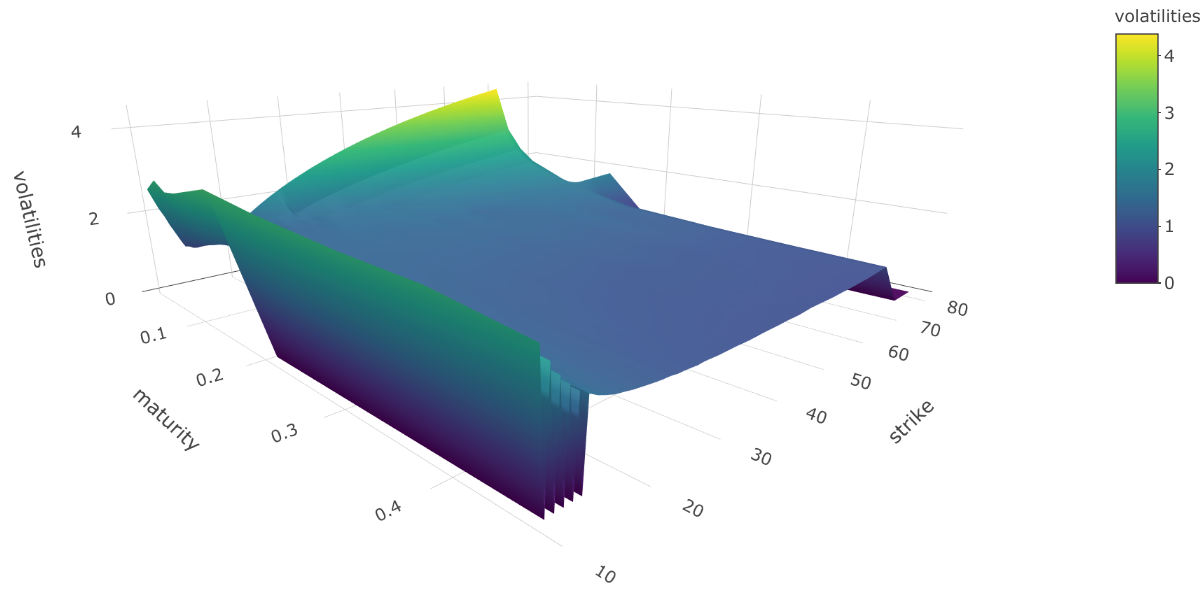
\includegraphics[scale=0.38]{fig1a.png}
\captionof{figure}{Superficie de volatilidad implícita de las opciones call del VIX del 1 de junio del 2016}
		\label{fig1.1}
\end{center}
Como mencionan \cite{gatheral_volatility_2018}, es conocido que en el mercado de valores, la forma general de la superficie de volatilidad es invariante bajo cambios de nivel y orientación, al menos en una primera aproximación. Lo anterior sugiere que la volatilidad es un proceso homogéneo en el tiempo, además de ser independiente del strike.

Las visibles discontinuidades de la \cref{fig1.1} se deben únicamente a los strikes cuya volatilidad correspondiente es $0$, es decir, a la ausencia de opciones en el mercado de valores con los strikes indicados, sin embargo, de existir (o en su defecto, extrapolar), se observa que seguirían la tendencia de homogeneidad en el tiempo e independencia del strike.

Los modelos homogéneos en el tiempo convencionales, no se ajustan a la superficie de volatilidad. Los modelos de volatilidad estocástica convencionales, por otro lado, generan una estructura de términos de sesgo \textbf{ATM} (en el dinero) que es constante para $\tau$ pequeña y se comporta como una suma de exponenciales decrecientes para $\tau$ más grande.% Particularmente, la estructura temporal observada en la desviación de la volatilidad at-the-money (\textsl{ATM}) $(k = 0)$,

En \cite{fukasawa_asymptotic_2011}, se muestra que para el modelo de volatilidad estocástica
$$Z_{t}=r t-\frac{1}{2} \int_{0}^{t} g\left(Y_{s}^{n}\right)^{2} d s+\int_{0}^{t} g\left(Y_{s}^{n}\right)\left[\theta d W_{s}^{\prime}+\sqrt{1-\theta^{2}} d W_{s}\right],$$
donde $Y_s^n=y+\epsilon_nW_s^H$, $\theta\in(-1,1), y\in\mathbb R$ son constantes, $g$ una función de Borel, $W_s$ y $W'$ son Bm, se tiene un sesgo de volatilidad ATM de la forma $\psi(\tau)\sim \tau^{H -1/2}$, al menos para $\tau$ pequeño.

Lo anterior proporciona un contraejemplo a la creencia de que la explosión del smile de la volatilidad cuando $\tau\rightarrow 0$, como se ve en las \cref{fig1.1,fig1.2}, implica la presencia de saltos, como mencionan por ejemplo \cite{carr_what_2003}. Cabe mencionar que, para que un modelo del tipo analizado por \cite{fukasawa_asymptotic_2011} genere una superficie de volatilidad con una forma razonable, necesitaríamos tener un valor de $H$ cercano a cero.

Como veremos en la \cref{sec:2.5}, nuestras estimaciones empíricas de $H$ a partir de datos de series de tiempo, efectivamente son muy pequeñas. El modelo de volatilidad que especificaremos en la \cref{sec3.1}, impulsado por un fBm con $H <\frac{1}{2}$, tiene potencial de satisfacer  las propiedades observadas empíricamente en las series de tiempo de volatilidad, así como de poseer la forma de la superficie de volatilidad antes descrita.
\begin{center}
	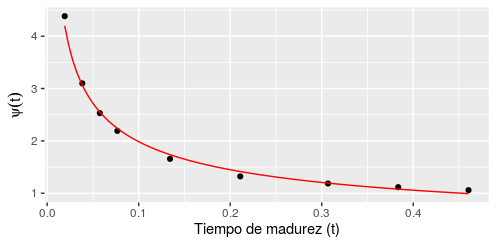
\includegraphics[scale=1.2]{fig2.png}
	\captionof{figure}{Estimaciones no paramétricas de los sesgos de volatilidad ATM del VIX con strike 70 al 1 de junio de 2016; la curva roja es la curva de ajuste $\psi(t)=0.7	t^{-0.45}$.}
	\label{fig1.2}
\end{center}
\section{La suavidad del proceso de volatilidad}\label{sec:1.2}
Es de utilidad en el análisis de regularidad de soluciones generalizadas a ecuaciones diferenciales parciales, hablar de la suavidad de tales procesos en el sentido de la regularidad de Hölder.
\begin{dfn}
Un proceso estocástico $X$ es $\beta-$Hölder continuo si existe una variable aleatoria finita $K$, a la que nos referimos como \textsl{constante de Hölder}, tal que
$$\sup_{s,t\in[0,1];s\neq t}\frac{|X_t-X_s|}{|t-s|^\beta}\leq K.$$
\end{dfn}
\textcolor{red}{Cambiar por la definición de Biagini 2008 pp4 Criterio de Kolmogorov}

Por lo anterior, de manera similar a lo estudiado en \cite{gatheral_volatility_2018}, comenzaremos estimando la suavidad de forma empírica para el proceso de volatilidad de los siguientes activos:
\begin{itemize}
	\item Los futuros DAX y Bund, para los cuales estimaremos la varianza integrada directamente a partir de datos de alta frecuencia, utilizando un estimador basado en el modelo con zonas de incertidumbre de \cite{robert_volatility_2012}, %citeauthor? para que imprima sin año
esto con los precios de entre las 10 y las 11 am (horario de Londres) de algunos días entre el 13 de Mayo del 2010 y el 1 de Agosto del 2014.
%lo siguiente si? o nel?
	\item Los índices S\&P y NASDAQ, para los cuales utilizaremos estimaciones de varianza previamente calculadas del Oxford-Man Institute of Quantitative Finance Realized Library, para algunos días entre el 3 de enero del 2000 y el 31 de marzo del 2014.
\end{itemize}
Supongamos que contamos con las observaciones discretas del proceso de volatilidad, en una retícula de tamaño $\Delta$ en el intervalo $[0,T]: \sigma_0,\sigma_\Delta,\ldots, \sigma_{k\Delta},\ldots$, $k\in\left\{0,\ldots, \lfloor \frac{T}{N}\rfloor\right\}$. Por simplicidad, tomemos $N=\lfloor \frac{T}{\Delta}\rfloor$ y para $q\geq 0$ definamos
$$m(q,\Delta)=\frac{1}{N}\sum_{k=1}^N \left|log(\sigma_{k\Delta})-log(\sigma_{(k-1)\Delta})\right|^q$$
Al igual que \cite{rosenbaum_etude_2007}, vamos a asumir que existen $s_q>0$ y $b_q>0$, tales que
\begin{align}
	N^{qs_q}m(q,\Delta)\buildrel \longrightarrow\over{\scriptscriptstyle{\Delta\rightarrow 0}}b_q\label{eqn:1.4}
\end{align}
La \cref{eqn:1.4} indica que el proceso de volatilidad pertenece al espacio de suavidad de Besov\footnote{Definido en el \cref{anx:A}} $\mathcal{B}_{q, \infty}^{s_{q}}$ y no pertenece a $\mathcal{B}_{q, \infty}^{s'_{q}}$, para $s'_q> s_q$. Por lo tanto, $s_q$ puede verse como la regularidad de la volatilidad cuando se mide en la norma $l_q$. En particular, las funciones en $\mathcal{B}_{q, \infty}^{s_{q}}$ para todo $q>0$ poseen  la propiedad de continuidad Hölder, con parámetro $h$ para cualquier $h <s$.

Suponiendo que los incrementos del proceso de log-volatilidad son estacionarios, además de que se cumplen las condiciones necesarias para aplicar la ley de los grandes números, $m(q,\Delta)$ puede verse como la versión empírica de
\begin{align}
\mathbb E\left[\left|log(\sigma_\Delta)-log(\sigma_0)\right|^q\right].\label{eqn:1.5}
\end{align}
El proceso de volatilidad no es directamente observable, así que no es posible calcular $m(q,\Delta)$ de manera exacta en la práctica, especialmente porque el menor $\Delta$ posible en la práctica es de $1$ día.  Aproximaremos las volatilidades para los mercados \textbf{spot} antes mencionados para una hora fija del día.

Como se mencionó anteriormente, para estimar la volatilidad en los futuros DAX y Bund,  usaremos el estimador de varianza integrada, el cual usa el modelo de zonas de incertidumbre de \cite{robert_volatility_2012} para 1248 días entre las fechas antes mencionadas, este modelo nos permite utilizar todos los datos de precios de frecuencia ultra alta para nuestra estimación, y así obtener estimaciones precisas en ventanas de tiempo cortas.

Para los índices S\&P y NASDAQ, aproximaremos las varianzas spot diarias utilizando las varianzas estimadas por el Oxford-Man Institute of Quantitative Finance Realized Library en 3540 días entre las fechas antes mencionadas.
%ve chido si metes lo siguiente o no, es medio claro usando una idea similar a sumas de riemann superiores.

%Dado que estas estimaciones de la varianza integrada son para todo el día de negociación, esperamos que las estimaciones de la suavidad del proceso de volatilidad estén sesgadas hacia arriba, siendo la integración una operación de regularización. Calculamos la extensión de este sesgo por simulación en la sección 3.4 y más cuantitativamente en el apéndice 3.
En lo consecuente, seguiremos usando la notación $m(q, \Delta)$ para referirnos a la aproximación de la volatilidad spot real, como se explicó anteriormente. Procederemos a estimar el parámetro de suavidad $s_q$ para cada $q$, al calcular $m(q,\Delta)$ para diferentes valores de $\Delta$ y haciendo un modelo de regresión para $log\; m (q,\Delta)$ en función de $log\:\Delta$. Notemos que para un determinado $\Delta$, varios $m (q ,\Delta)$ se pueden calcular según el punto de partida. Nuestro valor final de $m (q,\Delta)$ es el promedio simple de estos valores.
\subsection{Los futuros DAX y Bund}
El Futuro DAX es un contrato de futuro que tiene por subyacente al índice DAX, uno de los índices de la Bolsa de Fráncfort. Por otro lado, el futuro Bund es un bono sobre la deuda pública del Gobierno Federal alemán. Ambos se encuentran entre los activos con mayor liquidez del mundo, además, de acuerdo a \cite{Dayri_2005}, el modelo con zonas de incertidumbre utilizado para estimar la volatilidad se aplica bien a ellos.%agregalo a zotero, está en schoolar

Las gráficas de $log\; m (q,\Delta)$ vs $log\:\Delta$ para diferentes valores de $q$ son mostrado para el DAX en la \cref{fig1.3}, y para el Bund en la \cref{fig1.4}.
\begin{center}
	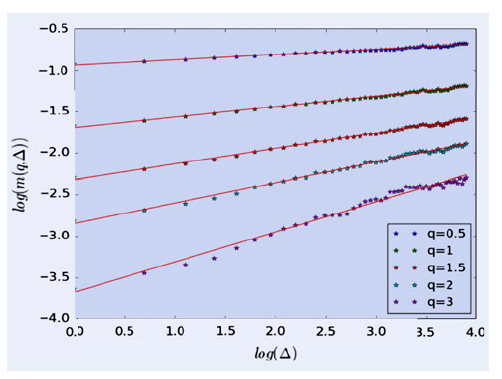
\includegraphics[scale=0.7]{fig3.png}
	\captionof{figure}{$log\; m(q, \Delta)$ como función de $log \:\Delta$ para el DAX.}
	\label{fig1.3}
\end{center}
\begin{center}
	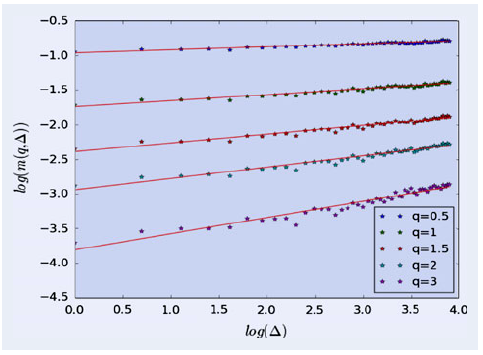
\includegraphics[scale=0.7]{fig4.png}
	\captionof{figure}{$log\; m(q, \Delta)$ como función de $log \:\Delta$ para el Bund.}
	\label{fig1.4}
\end{center}
Podemos observar en las \cref{fig1.3,fig1.4} que la regresión antes mencionada brinda una relación lineal bastante buena. Considerando la estacionariedad, ésto quiere decir que los incrementos de log-volatilidad poseen la siguiente propiedad de escala en esperanza
$$\mathbb E\left[\left|log(\sigma_\Delta)-log(\sigma_0)\right|^q\right]=b_q\Delta^{\xi_q},$$
que es una versión explícita de la \cref{eqn:1.5}, donde $\xi_q=qs_q>0$ es la pendiente de regresión. Más aún, el parámetro de suavidad $s_q$ parece no depender de $q$.

\section{??}
\textcolor{red}{No se como acortar lo siguiente}

En la \cref{sec:1.2} mostramos empíricamente que los incrementos de la volatilidad logarítmica de varios activos poseen una propiedad de escala con un parámetro de suavidad constante y que su distribución es cercana a la Gaussiana. Esto sugiere el modelo:
$$\sigma_t=\sigma exp\left(\nu W^H_t\right),$$
donde $W^H_t$ es un fBm de parámetro $H$ igual a la suavidad medida de volatilidad, $\nu,\sigma$ son constantes positivas.

Sin embargo, este modelo no es estacionario, lo cual sería deseable para garantizar que el modelo sea razonable para tiempos muy largos. Con motivo de lograr que el modelo sea estacionario, se buscó mejorar modelos como el presentado en la \cref{eq1.3}, modelando la volatilidad logarítmica como un proceso fraccionario de Ornstein–Uhlenbeck con una escala de tiempo de reversión muy larga, definido por la solución estacionaria de la ecuación diferencial estocástica
$$dX_t=\nu dW^H_t-\alpha(X_t-m)dt,$$
donde $m,\nu,\alpha\in\mathbb R$ y $\nu,\alpha>0$. Tal proceso fue estudiado por \cite{cheridito_fractional_2003}.
\textcolor{red}{Pendiente continuar, guiar con Cheridito}
\section{Las diferencias entre FSV y RFSV}\label{sec:2.4}
En \cite{comte_long_1998}, introducen el modelo de Volatilidad Estocástica Fraccionaria (FSV)
\textcolor{red}{Pendiente continuar, guiar con el Volatility is rought}
\chapter{El movimiento browniano fraccionario en finanzas}\label{ch:3}
En vista de la utilidad del modelo clásico de Black Scholes, en el cual utilizamos un fBm con parámetro de Hurst $H=\frac{1}{2}$, es natural pensar en la posibilidad de extender al fBm con $0<H<1$. Como se mencionó en \cref{lem1.2.9}, el fBm con $H>\frac{1}{2}$ posee cierta memoria o persistencia, mientras que con $H<\frac{1}{2}$ el fBm presenta ciertos efectos de turbulencias o antipersistencia, como se observó en la \ref{sec:2.4} y en similitud con el precio observado en el mercado nórdico liberado de electricidad, de acuerdo con \cite{simonsen_measuring_2003}.

Al remplazar sin cambios el Bm del modelo de Black Scholes por un fBm, a pesar de mantener cierta consistencia matemática, de acuerdo a \textcolor{red}{buscar bien las citas, creo que Cheridito}, cuando definimos la integral respecto al fBm como una integral por trayectorias, el mercado correspondiente presenta oportunidad de arbitraje.
\begin{theorem}
\end{theorem}
\section{???}\label{sec3.1}

%\chapter{Simulaciones}
%%%Para las simulaciones, el lamberton trae cosas útiles al final de pricing
\chapter*{Conclusiones}  

\appendix
\cleardoublepage
\addappheadtotoc\appendixpage
%%%%%%%%%%%%%%%%  Demostraciones?  %%%%%%%%%%%%%%%%%%%%
\chapter{Algunos resultados mencionados}\label{anx:A}
\begin{theorem}[Desigualdad de la suma de potencias]
\end{theorem}
\begin{dfn}[Espacios de Besov, \cite{rosenbaum_new_2011}]
	Sea $\Delta^h_n$ el operador definido por
	$$f(x)\mapsto\left\{\begin{matrix}f(x+h)-f(x)&\text{ si }n=1 \\
	\Delta^1_h(\Delta^{n-1}_h)f(x)\end{matrix}\right.$$
	El módulo $L^p$ de $n-$ésimo orden de suavidad de $f$ en $[0, 1]$ es
	$$\omega_{n}(f, t)_{p}=\sup _{|h| \leq t}\left\|\Delta_{h}^{n} f\right\|_{L^{p}\left(\Omega_{k, n}\right)},$$
	donde $\Omega_{h,n}=\{x\in[0,1]|\:x+hk\in[0,1],\: k=0,\ldots,n\}$. Para $1\leq p\leq \infty$, $s>0$, el espacio de Besov $\mathcal{B}_{p, \infty}^s([0,1])$ esta formado por las funciones $f\in L^p[0,1]$ tales que
	$$\sup_{j\geq 0}\left\{2^{sj}\omega_n(f,2^{-j})_p\right\}_{j\geq 0}<\infty$$
	donde $n\in\mathbb N$ y $s<n$.
	
	Es un espacio de Banach equipado con la norma
	$$||f||_{\mathcal{B}_{p, \infty}^s([0,1])}=||f||_{L^p}+\sup_{j\geq 0}\left\{2^{sj}\omega_n(f,2^{-j})_p\right\}_{j\geq 0}.$$
	Para una función real $f$ definida en $[0,1]$ y $0<p<\infty$, definamos $J^p_j(f)$ como
	$$J^p_j(f)=\sum_{k=1}^{2^j}\left|f(k2^{-j})-f(\{k-1\}2^{-j})\right|^p.$$
	Para $p=\infty$ es usual considerar la norma supremo.
\end{dfn}
\chapter{Códigos en R para los resultados presentados}
\section{La superficie de volatilidad}\label{anx:b1}
El código expuesto a continuación se encarga de importar los precios de opciones Call y Put al día 1 de junio del 2016 del índice VIX, éstos datos fueron obtenidos de manera gratuita del sitio \url{https://datashop.cboe.com/option-quotes}.
\lstinputlisting[language=R, basicstyle=\small, linerange={1-12,14-42}]{CargaDatos.R}
\newpage
A continuación se definen las funciones utilizadas en el análisis de los datos.
\lstinputlisting[language=R, basicstyle=\small]{FuncionesLlenado.R}
Se define y se llama a la función Plot3D, la cual muestra en un Viewer la superficie de volatilidad implícita para las opciones Call, mostrada en la \cref{fig1.1}.
\lstinputlisting[language=R, basicstyle=\small, linerange={1-32}]{Superficies.R}

\section{Estimaciones no paramétricas}
El siguiente código es utilizado para brindar una estimación no paramétrica de los sesgos de volatilidad.
\lstinputlisting[language=R]{NoParametrica.R}

\bibliographystyle{apalike-modified}
\bibliography{MibibliotecaC}
\backmatter%@sglvgdor
\end{document}